

\documentclass[12pt,a4paper]{article}


\setcounter{secnumdepth}{0}

\usepackage[utf8]{inputenc}
\usepackage[T1]{fontenc}
\usepackage[english]{babel}
\usepackage{geometry}
\usepackage{graphicx}
\usepackage{booktabs}
\usepackage{longtable}
\usepackage{array}
\usepackage{xcolor}
\usepackage{hyperref}
\usepackage{enumitem}
\usepackage{listings}
\usepackage{caption}
\usepackage{float}

\geometry{margin=2.5cm}


\definecolor{f1red}{RGB}{225,6,0}
\definecolor{darkgray}{RGB}{40,40,40}
\definecolor{lightgray}{RGB}{245,245,245}



\hypersetup{
	colorlinks=true,
	linkcolor=f1red,
	urlcolor=f1red,
	citecolor=f1red
}

% ------------------------------------------------------------
% Document
% ------------------------------------------------------------
\title{\textbf{Tableau Implementation for the F1 DW}\\
	\large Dashboard 1: Competitive Balance Overview}
\author{Giuseppe Rudi}
\date{May 2026}

\begin{document}
	
	\maketitle
	
	\tableofcontents
	\newpage
	

	\section{Purpose of this Document}

	The previous visualization document defined the analytical idea, the dashboard structure, and the storytelling logic of the Formula 1 Data Warehouse project.
	This document has a different purpose.
	It describes the practical and implementation-oriented steps used to build the dashboards in Tableau Public.
	
	The goal is therefore not to explain only \textit{which} charts should be created, but to document \textit{how} they are created in practice, starting from the exported CSV files of the Data Warehouse.
	
	

	

	\section{Input Data}

	
	The Formula 1 Data Warehouse was implemented in PostgreSQL.
	However, Tableau Public does not support a direct connection to a PostgreSQL database in the same way as Tableau Desktop with database connectors.
	For this reason, the warehouse tables were exported as CSV files and imported into Tableau Public as text files.
	


	\subsection{CSV Import Settings}

	
	Each CSV file was imported in Tableau using the text file connector.
	The following settings were used to avoid incorrect parsing of the files:
	
	\begin{longtable}{p{5cm} p{8cm}}
		\toprule
		\textbf{Setting} & \textbf{Value} \\
		\midrule
		Field separator & Comma \\
		Text qualifier & None \\
		Character set & UTF-8 \\
		Locale & English (United Kingdom) \\
		Field names & First row contains field names \\
		\bottomrule
	\end{longtable}
	

	
	% ============================================================
	\subsection{Logical Relationships Between CSV Tables}
	% ============================================================
	
	After importing the CSV files, the tables were connected in Tableau using logical relationships.
	
	The relationship structure used for the first dashboard is the following:
	
	
	\begin{figure}[H]
		\centering
		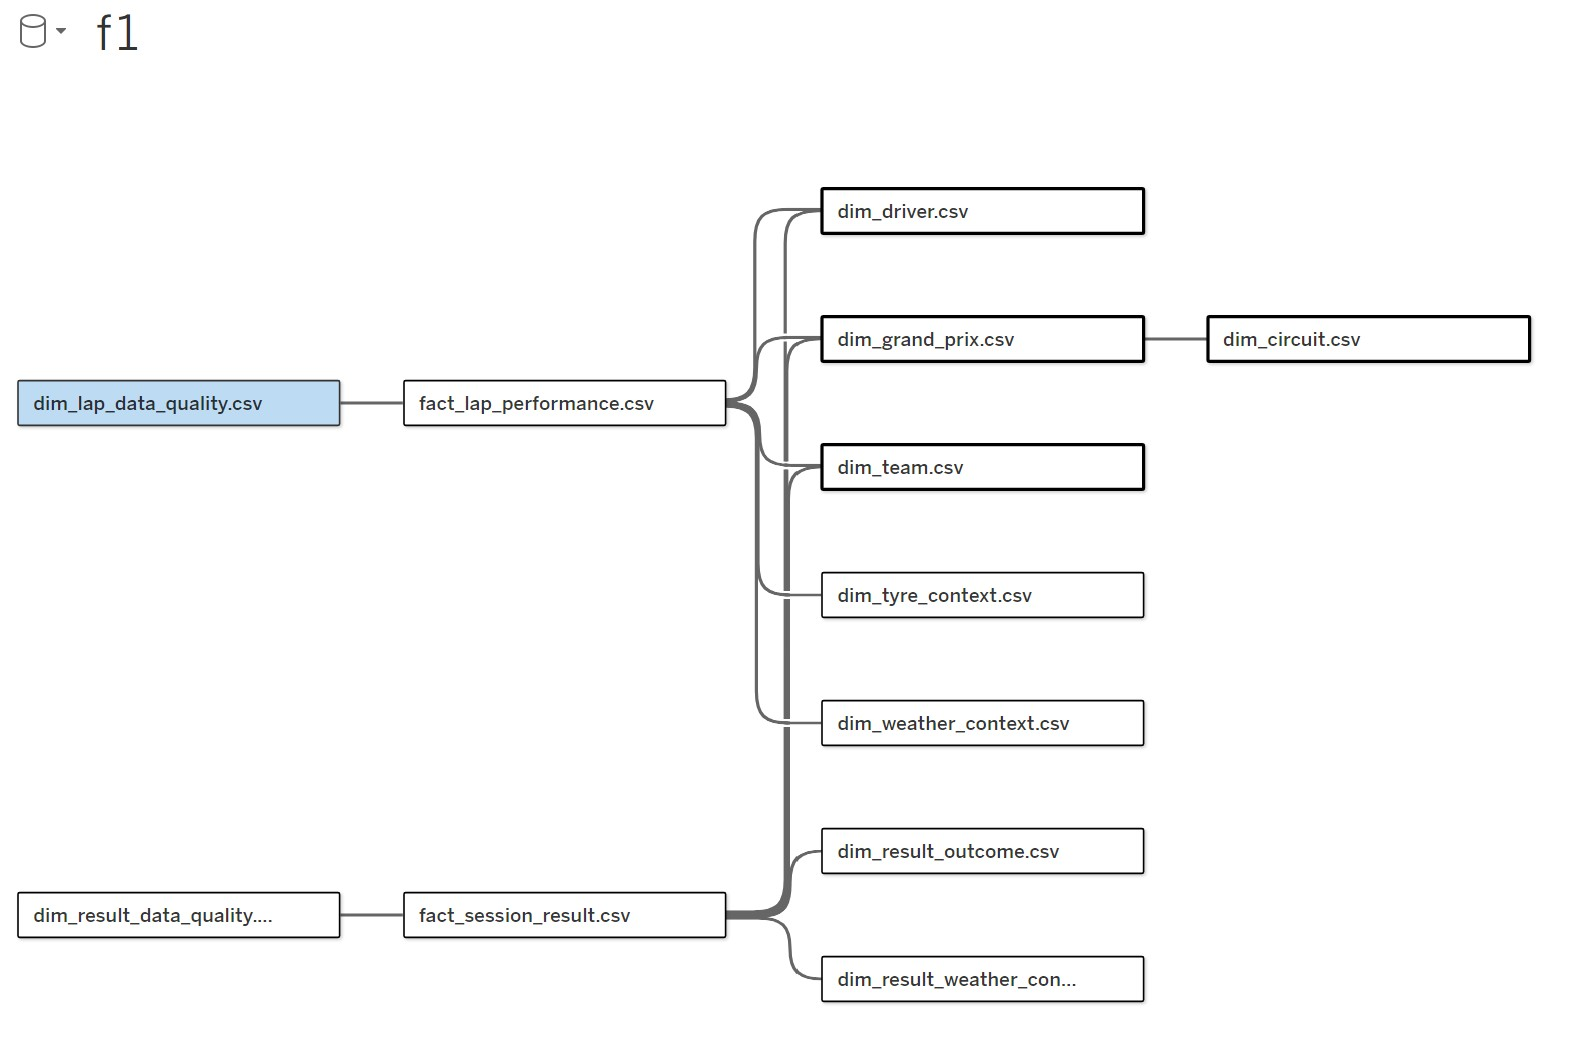
\includegraphics[width=0.95\textwidth]{images/tableau_relationship.jpg}
		\label{fig:dashboard1_overview}
	\end{figure}
	

	% ============================================================
	\section{General Analytical Filtering Strategy}
	% ============================================================
	
	All dashboards in the Tableau story are based on a controlled and interpretable analytical subset.
	However, the visualization system does not apply the same quality filters to every worksheet in a rigid way.
	
	This distinction is important because the Data Warehouse includes dedicated data quality dimensions, such as
	\texttt{dim\_lap\_data\_quality} for the Lap Performance fact and
	\texttt{dim\_result\_data\_quality} for the Session Result fact.
	
	The purpose of these dimensions is not to remove every record with any data quality issue from all analyses.
	Instead, they allow each dashboard and each worksheet to select only the records that are reliable for the specific analytical question being answered.
	
	For example, a lap with a speed information issue should not be used in a speed-based chart, but it may still be valid for a lap-time comparison if the lap time is present and reliable.
	Similarly, a lap with a sector information issue should be excluded from sector-based charts, but it does not necessarily need to be excluded from charts that only use complete lap time.
	The same logic applies to result-level analyses: a session result with a qualifying information issue should not be used for complete qualifying-time analysis, but it may still be usable in race-context or classification-based views when the required information is available.
	
	For this reason, the Tableau implementation uses two different levels of filters:
	
	\begin{itemize}[leftmargin=1.2cm]
		\item \textbf{global storytelling filters}, applied across the dashboards because they define the scope of the Formula 1 story;
		\item \textbf{chart-specific quality filters}, applied only to the worksheets where a specific type of information is required.
	\end{itemize}
	
	% ------------------------------------------------------------
	\subsection{Global Storytelling Filters}
	% ------------------------------------------------------------
	
	The global filters define the general analytical scope of the Tableau story.
	They are shared across the dashboards whenever possible, because all dashboards are part of the same narrative about the competitive balance between Ferrari, Red Bull, and Mercedes across the 2021 and 2022 seasons.
	
	\begin{longtable}{p{5cm} p{9cm}}
		\toprule
		\textbf{Filter} & \textbf{Default Value} \\
		\midrule
		Team & Ferrari, Red Bull, Mercedes \\
		Season & 2021 and 2022 \\
		Session Type & Qualifying and Race, depending on the dashboard \\
		Grand Prix & All selected Grand Prix events \\
		Circuit Category & All circuit categories by default \\
		Tyre Compound & Soft, Medium, Hard by default \\
		Rain Flag & False for the main dry-performance storytelling \\
		Track Status Category & AllClear for clean-lap performance comparisons \\
		\bottomrule
	\end{longtable}
	
	These filters are analytical filters, not cleaning rules.
	A record excluded by these filters is not necessarily wrong or invalid.
	It may simply be outside the controlled comparison required by the main storytelling.
	
	For example, wet laps, Safety Car laps, Virtual Safety Car laps, in-laps, out-laps, and pit-affected laps may be valid Formula 1 observations.
	However, they are not always suitable for the main comparison of clean car performance between teams.
	
	% ------------------------------------------------------------
	\subsection{Chart-Specific Quality Filters}
	% ------------------------------------------------------------
	
	The quality flags derived during the Data Cleaning phase are used selectively.
	They are not always applied as global dashboard filters.
	Instead, they are activated only when the corresponding type of information is necessary for a specific worksheet.
	
	This design choice is important because the Data Warehouse preserves records that may still be useful for some analyses, even if they are not suitable for others.
	
	\begin{longtable}{p{6cm} p{8cm}}
		\toprule
		\textbf{Lap Quality Flag} & \textbf{When It Is Used as a Filter} \\
		\midrule
		
		\texttt{has\_sector\_information\_issue}
		& Applied only in charts that use sector times, such as Sector 1, Sector 2, and Sector 3 performance comparisons. \\
		
		\texttt{has\_speed\_information\_issue}
		& Applied only in charts that use speed indicators, such as speed trap, finish-line speed, or straight-line speed analysis. \\
		
		\texttt{has\_tyre\_information\_issue}
		& Applied only in charts that compare performance by tyre compound, tyre life class, or tyre set status. \\
		
		\texttt{has\_weather\_information\_issue}
		& Applied only in charts that use weather context, such as air temperature, track temperature, wind speed, or rain-related analysis. \\
		
		\texttt{has\_track\_status\_issue}
		& Applied when the chart requires a reliable track-status interpretation. \\
		
		\texttt{has\_pit\_information\_issue}
		& Applied only when the chart needs to distinguish normal laps, in-laps, out-laps, and pit-affected laps. \\
		
		\bottomrule
	\end{longtable}
	
	For result-level analyses, the same principle is applied to the quality flags contained in
	\texttt{dim\_result\_data\_quality}.
	
	\begin{longtable}{p{6cm} p{8cm}}
		\toprule
		\textbf{Result Quality Flag} & \textbf{When It Is Used as a Filter} \\
		\midrule
		
		\small{has\_qualifying\_information\_issue}
		& Applied only in charts that require complete qualifying information, such as Q1, Q2, Q3, or qualifying-position analysis. \\
		
		\footnotesize{has\_race\_context\_information\_issue}
		& Applied only in charts that require complete race-context information, such as points, laps completed, race status, or race-time analysis. \\
		
		\bottomrule
	\end{longtable}
	
	This approach preserves more analytical information than a rigid global exclusion strategy.
	The Data Warehouse does not discard a lap or a result only because one specific information area is incomplete.
	Instead, the record remains available for the analyses that it can still support.
	
	Therefore, each dashboard applies the filters that are coherent with its specific analytical goal.
	For example, the circuit and sector dashboard uses sector quality filters, while the tyre and straight-line performance dashboard uses tyre and speed quality filters.
	The qualifying and race dashboard uses result quality filters only when the chart depends on complete qualifying or race-context information.
	
	This filtering strategy makes the Tableau implementation more transparent, more flexible, and more faithful to the design of the Data Warehouse.
	
	
	% ============================================================
	\section{General Tableau Field Configuration}
	% ============================================================
	
	Before implementing the individual dashboards, some fields were configured at workbook level.
	These configurations are not specific to Dashboard 1, because they are reused across the whole Tableau story.
	
	In particular, two aspects required special attention:
	
	\begin{itemize}[leftmargin=1.2cm]
		\item the definition of the selected top-team subset;
		\item the configuration of season and team fields for correct filtering and visual consistency.
	\end{itemize}
	
	
	% ------------------------------------------------------------
	\subsection{Team Color Configuration}
	% ------------------------------------------------------------
	
	The field \texttt{Team Name} is used in several worksheets as a color dimension.
	By default, Tableau assigns automatic colors to categorical values.
	However, these automatic colors do not correspond to the real visual identity of Formula 1 teams.
	
	For example, Tableau may assign green to Ferrari or brown to Red Bull Racing.
	This would be misleading and visually inconsistent with the Formula 1 theme of the project.
	
	For this reason, team colors were manually configured at workbook level.
	The objective is to ensure that every chart uses the same color for the same team across all dashboards.
	
	The selected colors are:
	
	\begin{longtable}{p{5cm} p{4cm} p{4cm}}
		\toprule
		\textbf{Team} & \textbf{Color Meaning} & \textbf{Hex Code} \\
		\midrule
		Ferrari & Ferrari red & \texttt{\#DC0000} \\
		Red Bull Racing & Red Bull blue & \texttt{\#1E41FF} \\
		Mercedes & Petronas turquoise & \texttt{\#00D2BE} \\
		\bottomrule
	\end{longtable}
	
	In Tableau, this configuration was applied through the default color properties of the field:
	
	\begin{quote}
		\texttt{Team Name} $\rightarrow$ \texttt{Default Properties} $\rightarrow$ \texttt{Color}
	\end{quote}
	
	After this configuration, every time \texttt{Team Name} is placed on the Color mark, Tableau reuses the selected Formula 1-inspired colors.
	
	This is important because color consistency helps the user read the dashboards more quickly.
	Ferrari, Red Bull Racing, and Mercedes keep the same visual identity in every worksheet and dashboard.
	
	
	% ------------------------------------------------------------
	\subsection{Season Year Configuration}
	% ------------------------------------------------------------
	
	The field \texttt{season\_year} is stored in the Data Warehouse as a numerical value.
	However, in Tableau it must not be interpreted as a continuous numerical measure.
	
	From an analytical point of view, \texttt{season\_year} is a categorical time attribute.
	In this project, it has two relevant values:
	
	\begin{itemize}[leftmargin=1.2cm]
		\item 2021;
		\item 2022.
	\end{itemize}
	
	Therefore, it should be used as a discrete dimension, not as a continuous measure.
	
	If Tableau imports \texttt{season\_year} as a green field, this means that it is being interpreted as continuous.
	In that case, Tableau may show the season filter as a range slider.
	This is not appropriate for this project, because the user should be able to select 2021, 2022, or both seasons as distinct categorical values.
	
	For this reason, the field was configured as follows:
	
	\begin{quote}
		\texttt{Season Year} $\rightarrow$ \texttt{Convert to Dimension}
	\end{quote}
	
	and then:
	
	\begin{quote}
		\texttt{Season Year} $\rightarrow$ \texttt{Convert to Discrete}
	\end{quote}
	
	After this configuration, \texttt{Season Year} appears as a blue discrete dimension in Tableau.
	
	The season filter can then be displayed as:
	
	\begin{quote}
		\texttt{Show Filter} $\rightarrow$ \texttt{Multiple Values Dropdown}
	\end{quote}
	
	or:
	
	\begin{quote}
		\texttt{Show Filter} $\rightarrow$ \texttt{Multiple Values List}
	\end{quote}
	
	This allows the user to select:
	
	\begin{itemize}[leftmargin=1.2cm]
		\item only 2021;
		\item only 2022;
		\item both 2021 and 2022.
	\end{itemize}
	
	This configuration is used across the dashboards because the comparison between the 2021 and 2022 seasons is one of the central elements of the storytelling.
	
	% ============================================================
	\section{Dashboard 1: Competitive Balance Overview}
	% ============================================================
	
	\subsection{Analytical Role of the Dashboard}
	
	The first dashboard is designed as the opening page of the Tableau story.
	Its role is to provide a high-level answer to the main business question:
	
	\begin{quote}
		\textit{How did the competitive balance among Ferrari, Red Bull, and Mercedes change from 2021 to 2022?}
	\end{quote}
	
	The dashboard does not aim to explain all technical causes of the observed changes.
	Instead, it shows whether there is evidence of a change in the competitive order between the two seasons.
	More detailed explanations about session context, circuit characteristics, sector behaviour, tyre compounds, and speed indicators are developed in the following dashboards.
	
	For this reason, the first dashboard mainly uses the \texttt{fact\_session\_result} table.
	This fact is more suitable for a high-level overview because it contains session-level outcomes such as points, final positions, qualifying positions, race classifications, and Grand Prix-level results.
	
	The \texttt{fact\_lap\_performance} table is used only as supporting evidence.
	It provides a clean lap-performance comparison, but the detailed lap-level interpretation is left to the later dashboards.
	
	
	\subsection{Team Scope and Interaction}
	
	The dashboard is initially configured to focus on Ferrari, Red Bull, and Mercedes.
	These teams represent the selected top-team subset used by the main storytelling.
	
	The user can interact with the team filter, but only within this selected subset.
	This means that the user can compare all three teams together or select smaller combinations, such as Ferrari versus Red Bull or Red Bull versus Mercedes.
	Other teams are not included in the main dashboard interaction because the purpose of this visualization is not to provide a fully open exploration of the entire Formula 1 grid, but to tell a controlled story about the competitive balance among the selected top teams.
	
	This choice preserves the narrative focus of the dashboard while still allowing a useful level of interactivity.
	
	\subsection{Fixed Scope Bar}
	
	At the top of the dashboard, a fixed scope bar is displayed.
	This bar is not an interactive filter.
	Its purpose is to communicate the analytical assumptions used by the dashboard.
	
	The scope bar contains the following information:
	
	\begin{quote}
		\textbf{Scope:} Top Teams \;|\; 2021--2022 \;|\; Dry Running for Lap Performance \;|\; All-Clear Track Status
	\end{quote}
	
	The dry-running and all-clear assumptions are especially relevant for the worksheets based on the \texttt{fact\_lap\_performance} table.
	For result-level charts based on \texttt{fact\_session\_result}, the dashboard focuses on official session outcomes for the selected teams and seasons.
	
	\subsection{Interactive Filters}
	
	The first dashboard contains only the interactive filters that are useful for the high-level competitive overview.
	
	\begin{longtable}{p{5cm} p{8cm}}
		\toprule
		\textbf{Filter} & \textbf{Purpose} \\
		\midrule
		Season & Allows the user to compare 2021 and 2022 together or focus on one season. \\
		Team & Allows the user to select or deselect Ferrari, Red Bull, and Mercedes. \\
		Session Type & Allows the user to distinguish between Qualifying and Race where applicable. \\
		Grand Prix & Allows the user to focus on one or more specific race weekends. \\
		\bottomrule
	\end{longtable}
	
	Filters related to circuit category, sector category, tyre compound, weather class, and speed indicators are not included in this dashboard.
	They are introduced only in the later dashboards where they support the specific analytical question.
	
	
	\subsection{Recommended Worksheets}
	
	The first dashboard is composed of a small number of high-level worksheets.
	
	\begin{longtable}{p{4cm} p{4cm} p{6cm}}
		\toprule
		\textbf{Worksheet} & \textbf{Main Source} & \textbf{Purpose} \\
		\midrule
		Total Race Points by Team and Season
		& \texttt{fact\_session\_result}
		& Shows the overall competitive outcome of each team in each season. \\
		
		Cumulative Points Trend by Grand Prix
		& \texttt{fact\_session\_result}
		& Shows how the competitive balance evolved across the season calendar. \\
		
		Average Race Position by Team and Season
		& \texttt{fact\_session\_result}
		& Provides a complementary view of consistency, where lower average position means better performance. \\
		
		Qualifying vs Race Summary Matrix
		& \texttt{fact\_session\_result}
		& Gives a compact preview of whether the change appears differently in Qualifying and Race sessions. \\
		
		Supporting Clean Lap Gap
		& \texttt{fact\_lap\_performance}
		& Adds lap-performance evidence without entering into detailed sector, tyre, or speed analysis. \\
		\bottomrule
	\end{longtable}
	
	% ------------------------------------------------------------
	\subsection{Step-by-Step Tableau Implementation}
	% ------------------------------------------------------------
	
	This subsection describes the practical steps followed in Tableau Public to build the first dashboard.
	The objective is to translate the analytical design into concrete Tableau worksheets and then combine them into the final dashboard layout.
	
	The implementation is based mainly on the \texttt{fact\_session\_result} table, because the first dashboard focuses on high-level competitive outcomes.
	The \texttt{fact\_lap\_performance} table is used only for one supporting worksheet related to clean lap-performance gaps.
	

	% ------------------------------------------------------------
	\subsubsection{Create the Fixed Scope Bar}
	% ------------------------------------------------------------
	
	Before creating the charts, a fixed scope bar is planned for the top part of the dashboard.
	This is not a Tableau filter.
	It is a static text element inserted in the dashboard layout.
	
	The text used is:
	
	\begin{quote}
		\textbf{Scope:} Top Teams \;|\; 2021--2022 \;|\; Dry Running for Lap Performance \;|\; All-Clear Track Status
	\end{quote}
	
	This scope bar informs the user about the assumptions of the dashboard.
	It is important because some filters, such as dry running and all-clear track status, are part of the analytical design and are not exposed as editable controls.
	
	% ------------------------------------------------------------
	\subsubsection{Worksheet -- Total Race Points by Team and Season}
	% ------------------------------------------------------------
	
	The first worksheet shows the total race points collected by each selected team in each season.
	This chart gives the most immediate high-level view of the competitive outcome.
	
	\paragraph{Data source.}
	The worksheet uses:
	
	\begin{quote}
		\texttt{fact\_session\_result}
	\end{quote}
	
	\paragraph{Chart type.}
	The selected Tableau chart type is a grouped bar chart.
	
	\paragraph{Tableau configuration.}
	
	\begin{longtable}{p{5cm} p{8cm}}
		\toprule
		\textbf{Tableau Area} & \textbf{Field} \\
		\midrule
		Columns & \texttt{season\_year} \\
		Rows & \texttt{SUM(points)} \\
		Color & \texttt{team\_name} \\
		Label & \texttt{SUM(points)} \\
		Filters & \texttt{Is Top Team = True} \\
		Filters & \texttt{session\_type = Race} \\
		Filters & \texttt{season\_year = 2021, 2022} \\
		\bottomrule
	\end{longtable}
	
	\paragraph{Formatting.}
	The bars are colored by team.
	The marks are labelled with the total number of points.
	The worksheet title is:
	
	\begin{quote}
		\textbf{Total Race Points by Team and Season}
	\end{quote}
	
	\paragraph{Interpretation.}
	This chart shows which team obtained the strongest race result output in each season.
	It is used as the main opening chart because points are easy to interpret and directly connected to competitive outcome.
	
	
	% ------------------------------------------------------------
	\subsubsection{Worksheet: Cumulative Points Gap to Leader}
	% ------------------------------------------------------------
	
	The second worksheet of Dashboard 1 was implemented as a cumulative gap chart.
	The goal of this visualization is to show how the competitive distance from the leading top team evolved during each season.
	
	The previous ranking-based version of the chart showed which team was first, second, or third after each Grand Prix.
	However, that visualization did not show the magnitude of the gap between the teams.
	For example, a team could remain second for many consecutive races, but the chart would not explain whether it was closing the gap to the leader or falling further behind.
	
	For this reason, the final implementation uses the cumulative points gap to the leading team.
	For each Grand Prix round, Tableau computes the cumulative race points of each selected team.
	Then, the leading team among Ferrari, Red Bull, and Mercedes is identified.
	Finally, the gap between each team and the leader is calculated.
	
	In this visualization:
	
	\begin{itemize}[leftmargin=1.2cm]
		\item a value equal to \texttt{0} identifies the current leader;
		\item negative values indicate how many points a team is behind the leader;
		\item a line moving downward means that the team is losing ground;
		\item a line moving upward toward zero means that the team is recovering points.
	\end{itemize}
	
	This chart is more informative than a pure cumulative ranking chart because it preserves the chronological interpretation of the championship battle while also showing the size of the competitive gap.
	
	% ------------------------------------------------------------
	\paragraph{Calculated Field: Race Points}
	% ------------------------------------------------------------
	
	The first calculated field isolates the points obtained in Race sessions.
	
	\begin{lstlisting}[basicstyle=\ttfamily\footnotesize]
		IF [Session Type] = "R" THEN [Points] END
	\end{lstlisting}
	
	This field was named:
	
	\begin{quote}
		\texttt{Race Points}
	\end{quote}
	
	The field is row-level and does not contain an aggregation.
	The aggregation is applied later in the worksheet.
	
	% ------------------------------------------------------------
	\paragraph{Calculated Field: Cumulative Team Points}
	% ------------------------------------------------------------
	
	The second calculated field computes the cumulative race points of each team along the Grand Prix sequence.
	
	\begin{lstlisting}[basicstyle=\ttfamily\footnotesize]
		RUNNING_SUM(SUM([Race Points]))
	\end{lstlisting}
	
	This field was named:
	
	\begin{quote}
		\texttt{Cumulative Team Points}
	\end{quote}
	
	The running sum is computed along \texttt{round\_number}.
	This means that, for each team and season, Tableau progressively accumulates the race points obtained from the first Grand Prix to the current round.
	
	% ------------------------------------------------------------
	\paragraph{Calculated Field: Cumulative Leader Points}
	% ------------------------------------------------------------
	
	The third calculated field identifies the highest cumulative points value among the selected top teams in each season and round.
	
	\begin{lstlisting}[basicstyle=\ttfamily\footnotesize]
		WINDOW_MAX([Cumulative Team Points])
	\end{lstlisting}
	
	This field was named:
	
	\begin{quote}
		\texttt{Cumulative Leader Points}
	\end{quote}
	
	The window maximum is computed across the selected teams within the same season and Grand Prix round.
	Therefore, it represents the cumulative points of the current leader among Ferrari, Red Bull, and Mercedes.
	
	% ------------------------------------------------------------
	\paragraph{Calculated Field: Gap To Cumulative Leader}
	% ------------------------------------------------------------
	
	The final calculated field computes the distance between each team and the current cumulative leader.
	
	\begin{lstlisting}[basicstyle=\ttfamily\footnotesize]
		[Cumulative Team Points] - [Cumulative Leader Points]
	\end{lstlisting}
	
	This field was named:
	
	\begin{quote}
		\texttt{Gap To Cumulative Leader}
	\end{quote}
	
	The leading team has a gap equal to \texttt{0}.
	The other teams have negative values, representing the number of points behind the leader.
	
	% ------------------------------------------------------------
	\paragraph{Worksheet Configuration}
	% ------------------------------------------------------------
	
	The worksheet was configured as a line chart.
	
	\begin{longtable}{p{5cm} p{8cm}}
		\toprule
		\textbf{Tableau Area} & \textbf{Field} \\
		\midrule
		Columns & \texttt{round\_number} \\
		Rows & \texttt{season\_year}, then \texttt{Gap To Cumulative Leader} \\
		Marks & Line \\
		Color & \texttt{team\_name} \\
		Path & \texttt{round\_number} \\
		Filters & \texttt{Is Top Team = True}, \texttt{Session Type = R}, \texttt{season\_year = 2021, 2022} \\
		Tooltip & \texttt{team\_name}, \texttt{event\_name}, \texttt{round\_number}, \texttt{Race Points}, \texttt{Cumulative Team Points}, \texttt{Gap To Cumulative Leader} \\
		\bottomrule
	\end{longtable}
	
	The field \texttt{round\_number} was used as a continuous field in order to create a smooth chronological line across the Grand Prix sequence.
	The field \texttt{season\_year} was placed in the Rows shelf before the gap measure.
	This creates two vertically separated panels: one for 2021 and one for 2022.
	
	This vertical layout was preferred over a side-by-side layout because it makes the comparison more readable inside the dashboard.
	If both seasons are selected, Tableau displays the two seasonal panels.
	If only one season is selected through the interactive filter, only the corresponding panel remains visible.
	
	% ------------------------------------------------------------
	\paragraph{Table Calculation Configuration}
	% ------------------------------------------------------------
	
	The measure \texttt{Gap To Cumulative Leader} depends on two nested table calculations.
	
	First, \texttt{Cumulative Team Points} uses a running sum.
	This calculation must be computed along the Grand Prix order:
	
	\begin{quote}
		\texttt{RUNNING\_SUM} $\rightarrow$ compute using \texttt{round\_number}
	\end{quote}
	
	Second, \texttt{Cumulative Leader Points} uses a window maximum.
	This calculation must compare the teams within the same season and round:
	
	\begin{quote}
		\texttt{WINDOW\_MAX} $\rightarrow$ compute using \texttt{team\_name}
	\end{quote}
	
	Conceptually, the calculation works as follows:
	
	\begin{itemize}[leftmargin=1.2cm]
		\item the running sum accumulates points across Grand Prix rounds;
		\item the window maximum identifies the current leader among the selected teams;
		\item the gap calculation subtracts the leader value from each team's cumulative value.
	\end{itemize}
	
	% ------------------------------------------------------------
	\paragraph{Reference Line}
	% ------------------------------------------------------------
	
	A horizontal reference line was added at value \texttt{0}.
	This line represents the current leader.
	
	The reference line was configured as follows:
	
	\begin{longtable}{p{5cm} p{8cm}}
		\toprule
		\textbf{Setting} & \textbf{Value} \\
		\midrule
		Scope & Per Pane \\
		Value & Constant \texttt{0} \\
		Label & \texttt{Leader} \\
		Tooltip & None \\
		\bottomrule
	\end{longtable}
	
	The reference line improves readability because every team line can be interpreted relative to the leader.
	A team on the zero line is leading the selected top-team group.
	A team below zero is behind the leader.
	
	% ------------------------------------------------------------
	\paragraph{Interpretation}
	% ------------------------------------------------------------
	
	The chart provides a clearer view of the competitive balance than a simple ranking chart.
	In the 2021 panel, the lines show how close Red Bull and Mercedes remained during the season, while Ferrari stayed further from the leadership battle.
	In the 2022 panel, the chart shows how Red Bull reached the leadership line and then maintained it, while Ferrari and Mercedes progressively moved further away from the leader.
	
	This makes the visualization suitable for the opening dashboard.
	It does not only show which team was leading, but also whether the other teams were gaining or losing ground during the season.
	

	\subsubsection{Worksheet 3 -- Average Race Position by Team and Season}
	% ------------------------------------------------------------
	
	The third worksheet provides a complementary view of race consistency.
	While points measure final reward, average position shows how consistently a team finished near the front.
	
	\paragraph{Data source.}
	The worksheet uses:
	
	\begin{quote}
		\texttt{fact\_session\_result}
	\end{quote}
	
	\paragraph{Chart type.}
	The selected chart type is a grouped bar chart or a slope chart.
	In the first implementation, a grouped bar chart is easier to read inside the dashboard.
	
	\paragraph{Tableau configuration.}
	
	\begin{longtable}{p{5cm} p{8cm}}
		\toprule
		\textbf{Tableau Area} & \textbf{Field} \\
		\midrule
		Columns & \texttt{season\_year} \\
		Rows & \texttt{AVG(position)} \\
		Color & \texttt{team\_name} \\
		Label & \texttt{AVG(position)} \\
		Filters & \texttt{Is Top Team = True} \\
		Filters & \texttt{session\_type = Race} \\
		Filters & \texttt{season\_year = 2021, 2022} \\
		\bottomrule
	\end{longtable}
	
	\paragraph{Important formatting note.}
	For this chart, lower values are better.
	For this reason, the title or subtitle must explicitly state:
	
	\begin{quote}
		\textit{Lower average position means better race classification.}
	\end{quote}
	
	\paragraph{Interpretation.}
	This chart prevents the dashboard from relying only on points.
	A team may score many points because of a few strong results, while average position gives a more stable indication of race classification consistency.
	
	% ------------------------------------------------------------
	\subsubsection{Step 7: Worksheet 4 -- Qualifying vs Race Summary Matrix}
	% ------------------------------------------------------------
	
	The fourth worksheet introduces a compact comparison between Qualifying and Race sessions.
	It does not yet provide the detailed explanation of session-specific performance.
	Instead, it works as a bridge toward the second dashboard.
	
	\paragraph{Data source.}
	The worksheet uses:
	
	\begin{quote}
		\texttt{fact\_session\_result}
	\end{quote}
	
	\paragraph{Chart type.}
	The selected Tableau chart type is a highlight table.
	
	\paragraph{Tableau configuration.}
	
	\begin{longtable}{p{5cm} p{8cm}}
		\toprule
		\textbf{Tableau Area} & \textbf{Field} \\
		\midrule
		Rows & \texttt{team\_name} \\
		Columns & \texttt{season\_year}, then \texttt{session\_type} \\
		Marks type & Square \\
		Color & \texttt{AVG(position)} \\
		Label & \texttt{AVG(position)} \\
		Filters & \texttt{Is Top Team = True} \\
		Filters & \texttt{season\_year = 2021, 2022} \\
		\bottomrule
	\end{longtable}
	
	\paragraph{Formatting.}
	The color scale is based on average position.
	The chart must clearly indicate that lower values represent better results.
	
	\paragraph{Interpretation.}
	This matrix gives an initial indication of whether the competitive change appears in both Qualifying and Race sessions.
	The detailed analysis of this distinction is then developed in Dashboard 2.
	
	% ------------------------------------------------------------
	\subsubsection{Step 8: Worksheet 5 -- Supporting Clean Lap Gap}
	% ------------------------------------------------------------
	
	The fifth worksheet uses lap-level data as supporting evidence.
	It does not replace the result-based interpretation of the first dashboard.
	Instead, it checks whether the high-level result pattern is also visible in clean lap-performance data.
	
	\paragraph{Data source.}
	The worksheet uses:
	
	\begin{quote}
		\texttt{fact\_lap\_performance}
	\end{quote}
	
	\paragraph{Required filters.}
	Since this worksheet uses lap-level performance, the following filters are applied:
	
	\begin{longtable}{p{5cm} p{8cm}}
		\toprule
		\textbf{Filter} & \textbf{Value} \\
		\midrule
		\texttt{Is Top Team} & True \\
		\texttt{lap\_type} & NormalLap \\
		\texttt{rain\_flag} & False \\
		\texttt{track\_status\_category} & AllClear \\
		\texttt{lap\_time\_ms} & Not null \\
		\bottomrule
	\end{longtable}
	
	The quality flags are not all applied globally.
	Only the flags required by the specific worksheet are used.
	For this chart, the essential condition is that lap time is available and that the lap belongs to the controlled clean-lap context.
	
	\paragraph{Calculated fields.}
	The chart uses the previously defined gap measure:
	
	\begin{lstlisting}[basicstyle=\ttfamily\footnotesize]
		[Team Avg Lap Time S] - [Best Team Avg Lap Time S]
	\end{lstlisting}
	
	\paragraph{Chart type.}
	The selected chart type is a grouped bar chart or slope chart.
	
	\paragraph{Tableau configuration.}
	
	\begin{longtable}{p{5cm} p{8cm}}
		\toprule
		\textbf{Tableau Area} & \textbf{Field} \\
		\midrule
		Columns & \texttt{season\_year} \\
		Rows & \texttt{AVG([Gap To Best Team S])} \\
		Color & \texttt{team\_name} \\
		Label & \texttt{AVG([Gap To Best Team S])} \\
		Filters & Top-team and clean-lap filters \\
		\bottomrule
	\end{longtable}
	
	\paragraph{Interpretation.}
	Lower values indicate that the team is closer to the best average lap performance in the same season, Grand Prix, and session context.
	This chart provides supporting evidence, while the main interpretation of Dashboard 1 remains result-based.
	
	% ------------------------------------------------------------
	\subsubsection{Step 9: Build the Dashboard Layout}
	% ------------------------------------------------------------
	
	After creating the worksheets, a new dashboard is created in Tableau and named:
	
	\begin{quote}
		\texttt{Dashboard 1 -- Competitive Balance Overview}
	\end{quote}
	
	The layout is organized using vertical and horizontal containers.
	
	The final structure is:
	
	\begin{verbatim}
		------------------------------------------------------------
		Dashboard title and main question
		------------------------------------------------------------
		Fixed scope bar
		------------------------------------------------------------
		Interactive filter bar
		------------------------------------------------------------
		Main result chart:
		Total Race Points by Team and Season
		------------------------------------------------------------
		Cumulative Points Trend by Grand Prix
		------------------------------------------------------------
		Average Race Position      Qualifying vs Race Matrix
		------------------------------------------------------------
		Supporting Clean Lap Gap
		------------------------------------------------------------
		Key message
		------------------------------------------------------------
	\end{verbatim}
	
	The title inserted at the top of the dashboard is:
	
	\begin{quote}
		\textbf{Competitive Balance Overview}
	\end{quote}
	
	The subtitle is:
	
	\begin{quote}
		\textit{How did the top-team balance change from 2021 to 2022?}
	\end{quote}
	
	% ------------------------------------------------------------
	\subsubsection{Step 10: Add the Final Dashboard Message}
	% ------------------------------------------------------------
	
	At the bottom of the dashboard, a short text box is added to guide interpretation.
	
	The suggested text is:
	
	\begin{quote}
		This dashboard provides a high-level view of the competitive balance between Ferrari, Red Bull, and Mercedes across the 2021 and 2022 seasons. Result-level charts show how the competitive outcome changed, while the lap-performance chart provides supporting evidence under clean running conditions.
	\end{quote}
	
	This message helps the user understand the role of the first dashboard.
	The dashboard answers the main question at a general level, while the following dashboards explain the technical and contextual reasons behind the observed change.
	
\end{document}
